\documentclass[14pts]{article}

\usepackage{graphicx}
\usepackage{url}
\usepackage{hyperref}
\hypersetup{colorlinks = true, citecolor = blue, linkcolor = blue, urlcolor = blue}

\usepackage{lipsum}

\usepackage[margin = 1in]{geometry}

\usepackage{amssymb}
\usepackage{amsmath}

\usepackage{caption}
\usepackage{subcaption}

\usepackage[perpage]{footmisc}
\renewcommand{\thefootnote}{\fnsymbol{footnote}}
%\footnote[number]{text}
%1 asterisk *
%2 dagger †
%3 double dagger ‡
%4 section symbol §
%5 paragraph ¶
%6 parallel lines ‖
%7 two asterisks **
%8 two daggers ††
%9 two double daggers ‡‡


% Using titlepage Environment instead of \maketitle
% \title{Visualizing functions using Python and Octave}
% \author{Atharva Aalok}
% \date{July 9, 2021}



\begin{document}
    \begin{titlepage}
        \begin{center}
            \rule{\textwidth}{1pt}\\
            \Huge
            \textbf{Visualizing \\ The Mandelbrot Set \\ and \\ The Lorenz Attractor }\\
            \rule{\textwidth}{1pt}
            \vfill
            
            \Large
            \textbf{Submitted by:}
            \medskip

            Atharva Aalok
            \vfill

            
\includegraphics[width = 2in]{Images/IITM_logo.svg.png}
            \vfill

            Department of Aerospace Engineering,
            \medskip

            Indian Institute of Technology Madras
            \vfill

            July 9, 2021

        \end{center}
    \end{titlepage}


    \renewcommand*\contentsname{Summary}
    \tableofcontents

    \pagebreak
    \section{Why use Python or Octave?}
    Helllo My name is Atharva\footnote[2]{the guy who created this} \\
    \lipsum[1-2]

    \pagebreak



    \section{The Mandelbrot Set}
    The Mandelbrot set is the set of all complex numbers $ c $ for which $z_{n}$ defined by the iteration $ z_{n+1} = z_{n}^2 + c $ with $ z_{0} = 0 $ remains bounded in absolute value.
    It can be shown that for $ c $ to lie in the Mandelbrot set the magnitude of $ z_{n} $ should never exceed $ 2 $.

    i.e. if M denotes the Mandelbrot set then
    \[ M = \{c : c \in \mathbb{C} \ \land \ z_{n+1}:=z_{n}^2 + c \ \land \ \exists \ m \in \mathbb{N} \ \text{such that} \lim_{n \to \infty} z_{n} \leq m \} \]

    To get an idea of how the set looks like we wrote a Python program that plots points on the complex plane whose magnitude remains less than equal to 2 after a certain threshold value of iterations under the above defined rule.\footnote[2]{For the Python codes used to generate the plot refer \url{mygithubpage}}
    \bigskip

    
    \begin{figure}[!h]
        \centering
        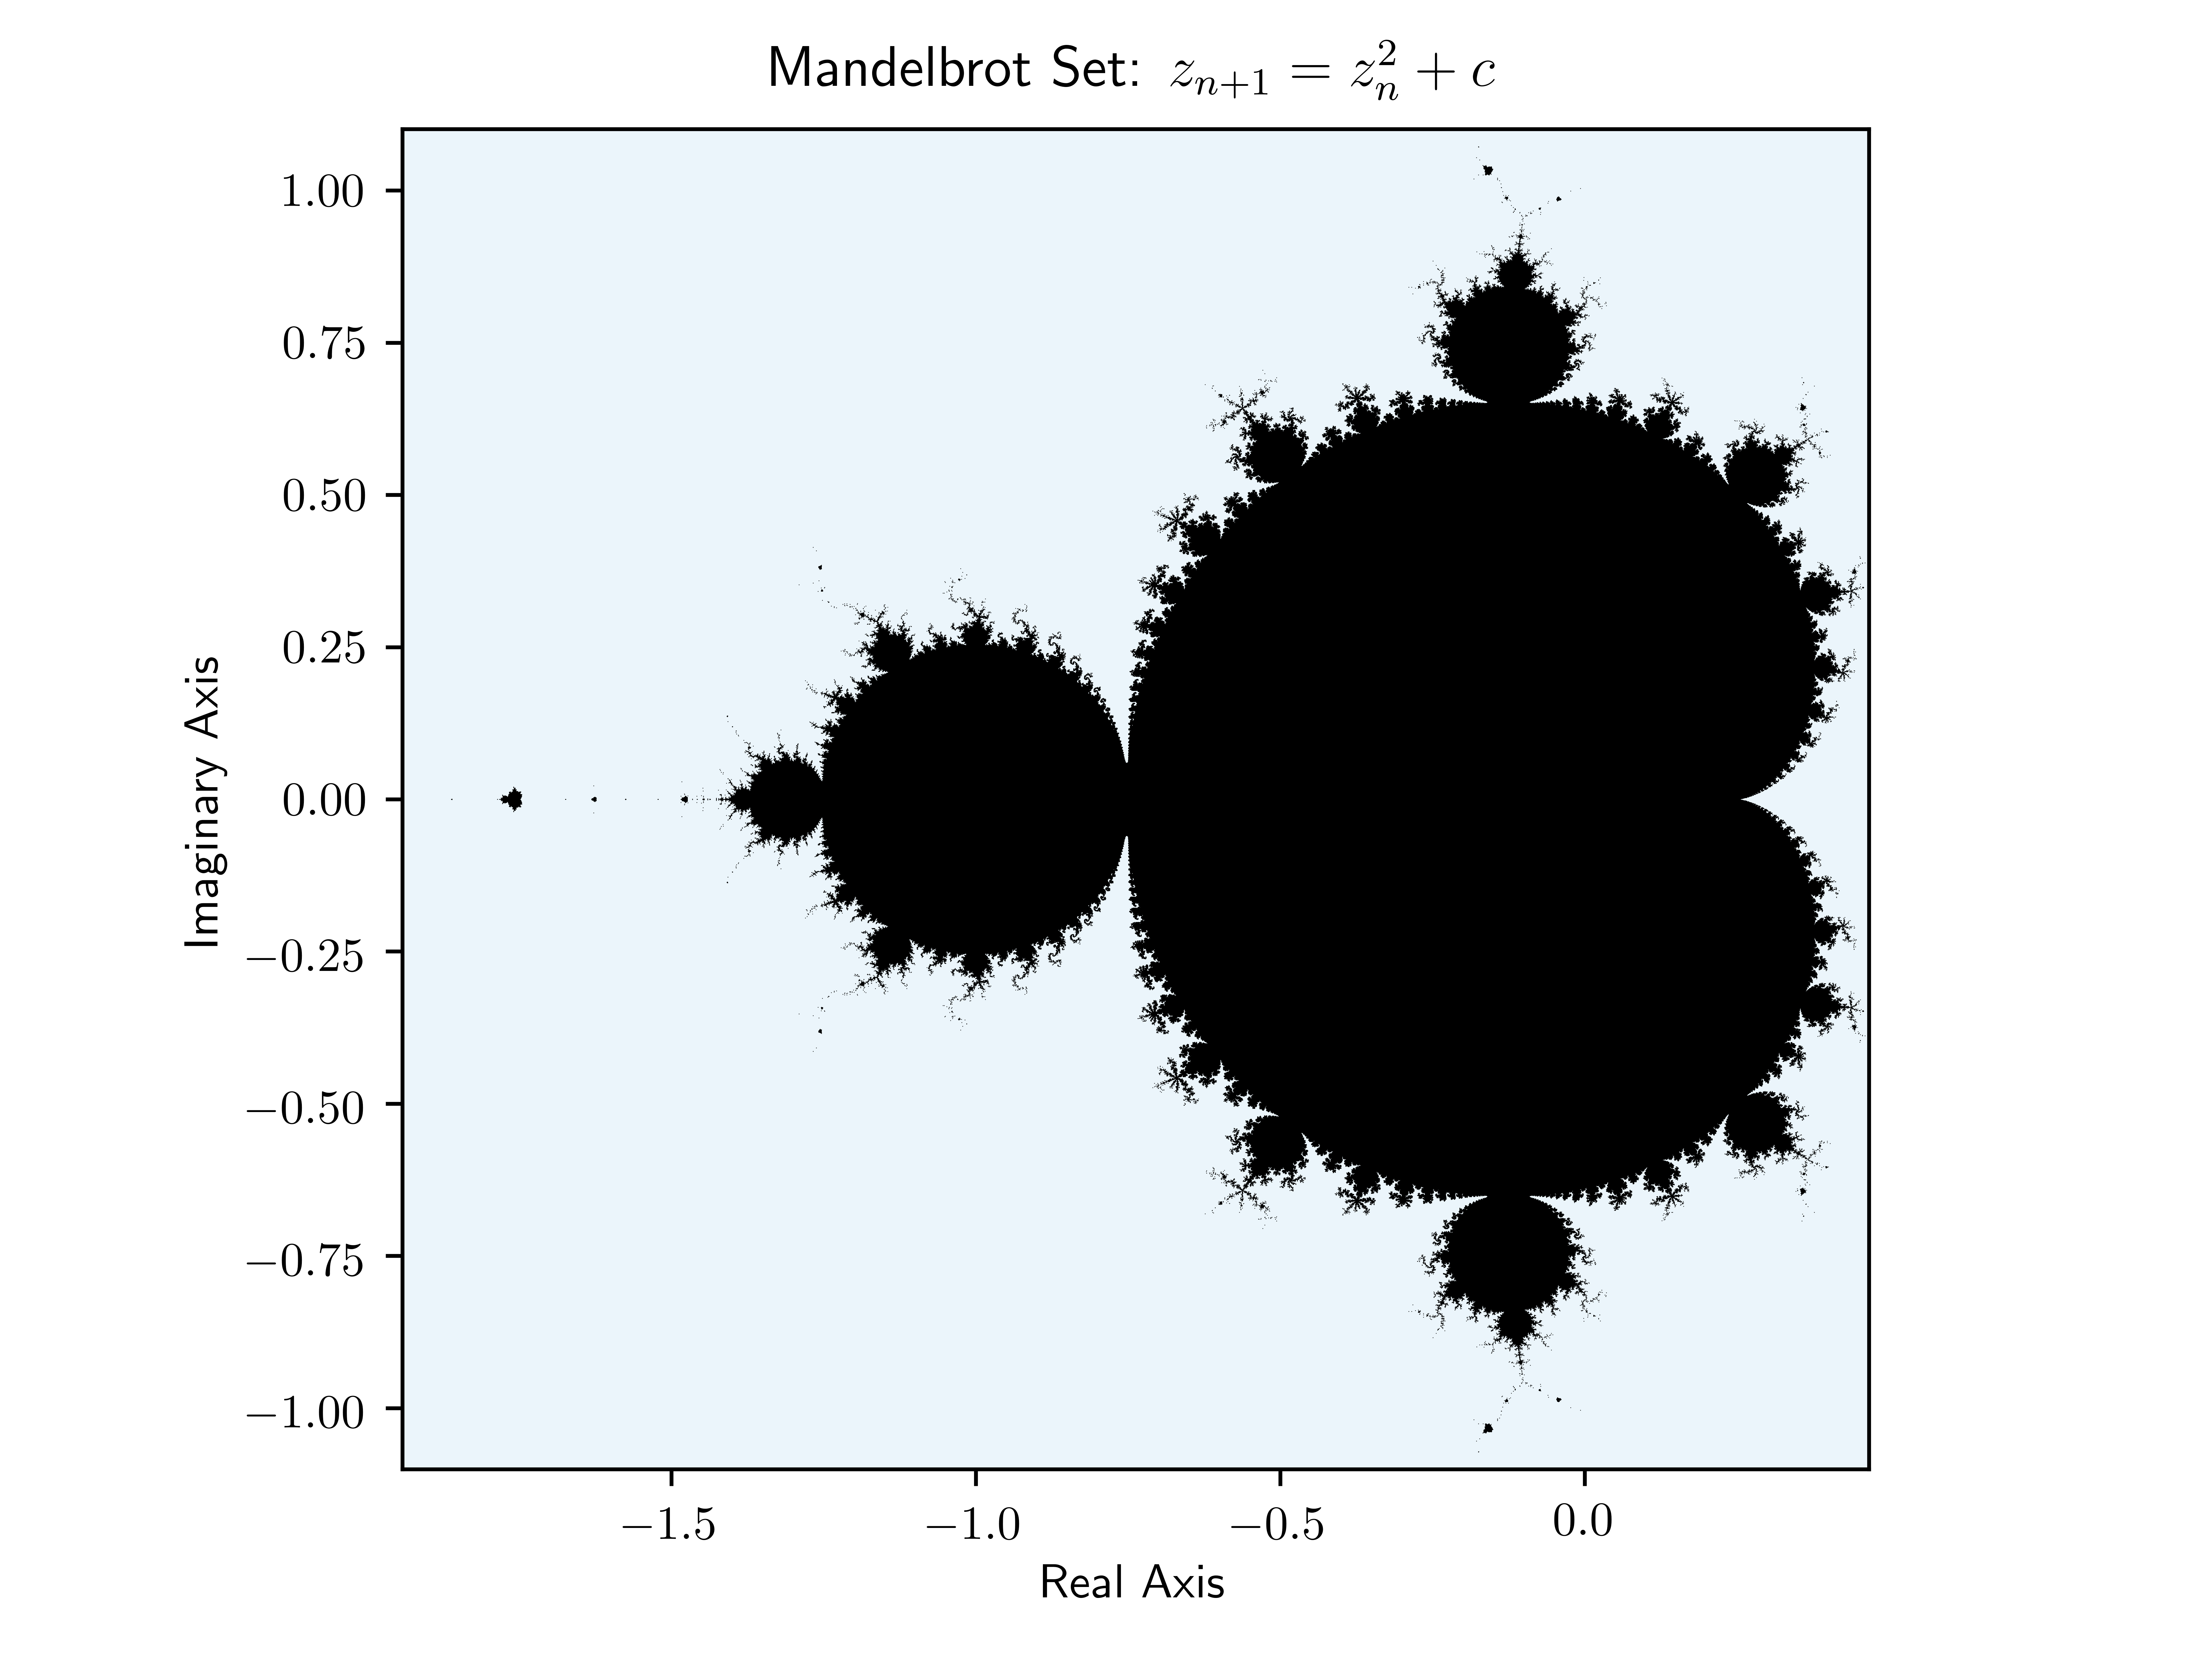
\includegraphics[width = \textwidth]{Images/Mandelbrot_set.png}
        \caption{The Mandelbrot Set}
        \label{fig:Mandelbrot}
    \end{figure}


    \begin{figure}[!h]
        \centering
        \begin{subfigure}{.8\textwidth}
            %\centering
            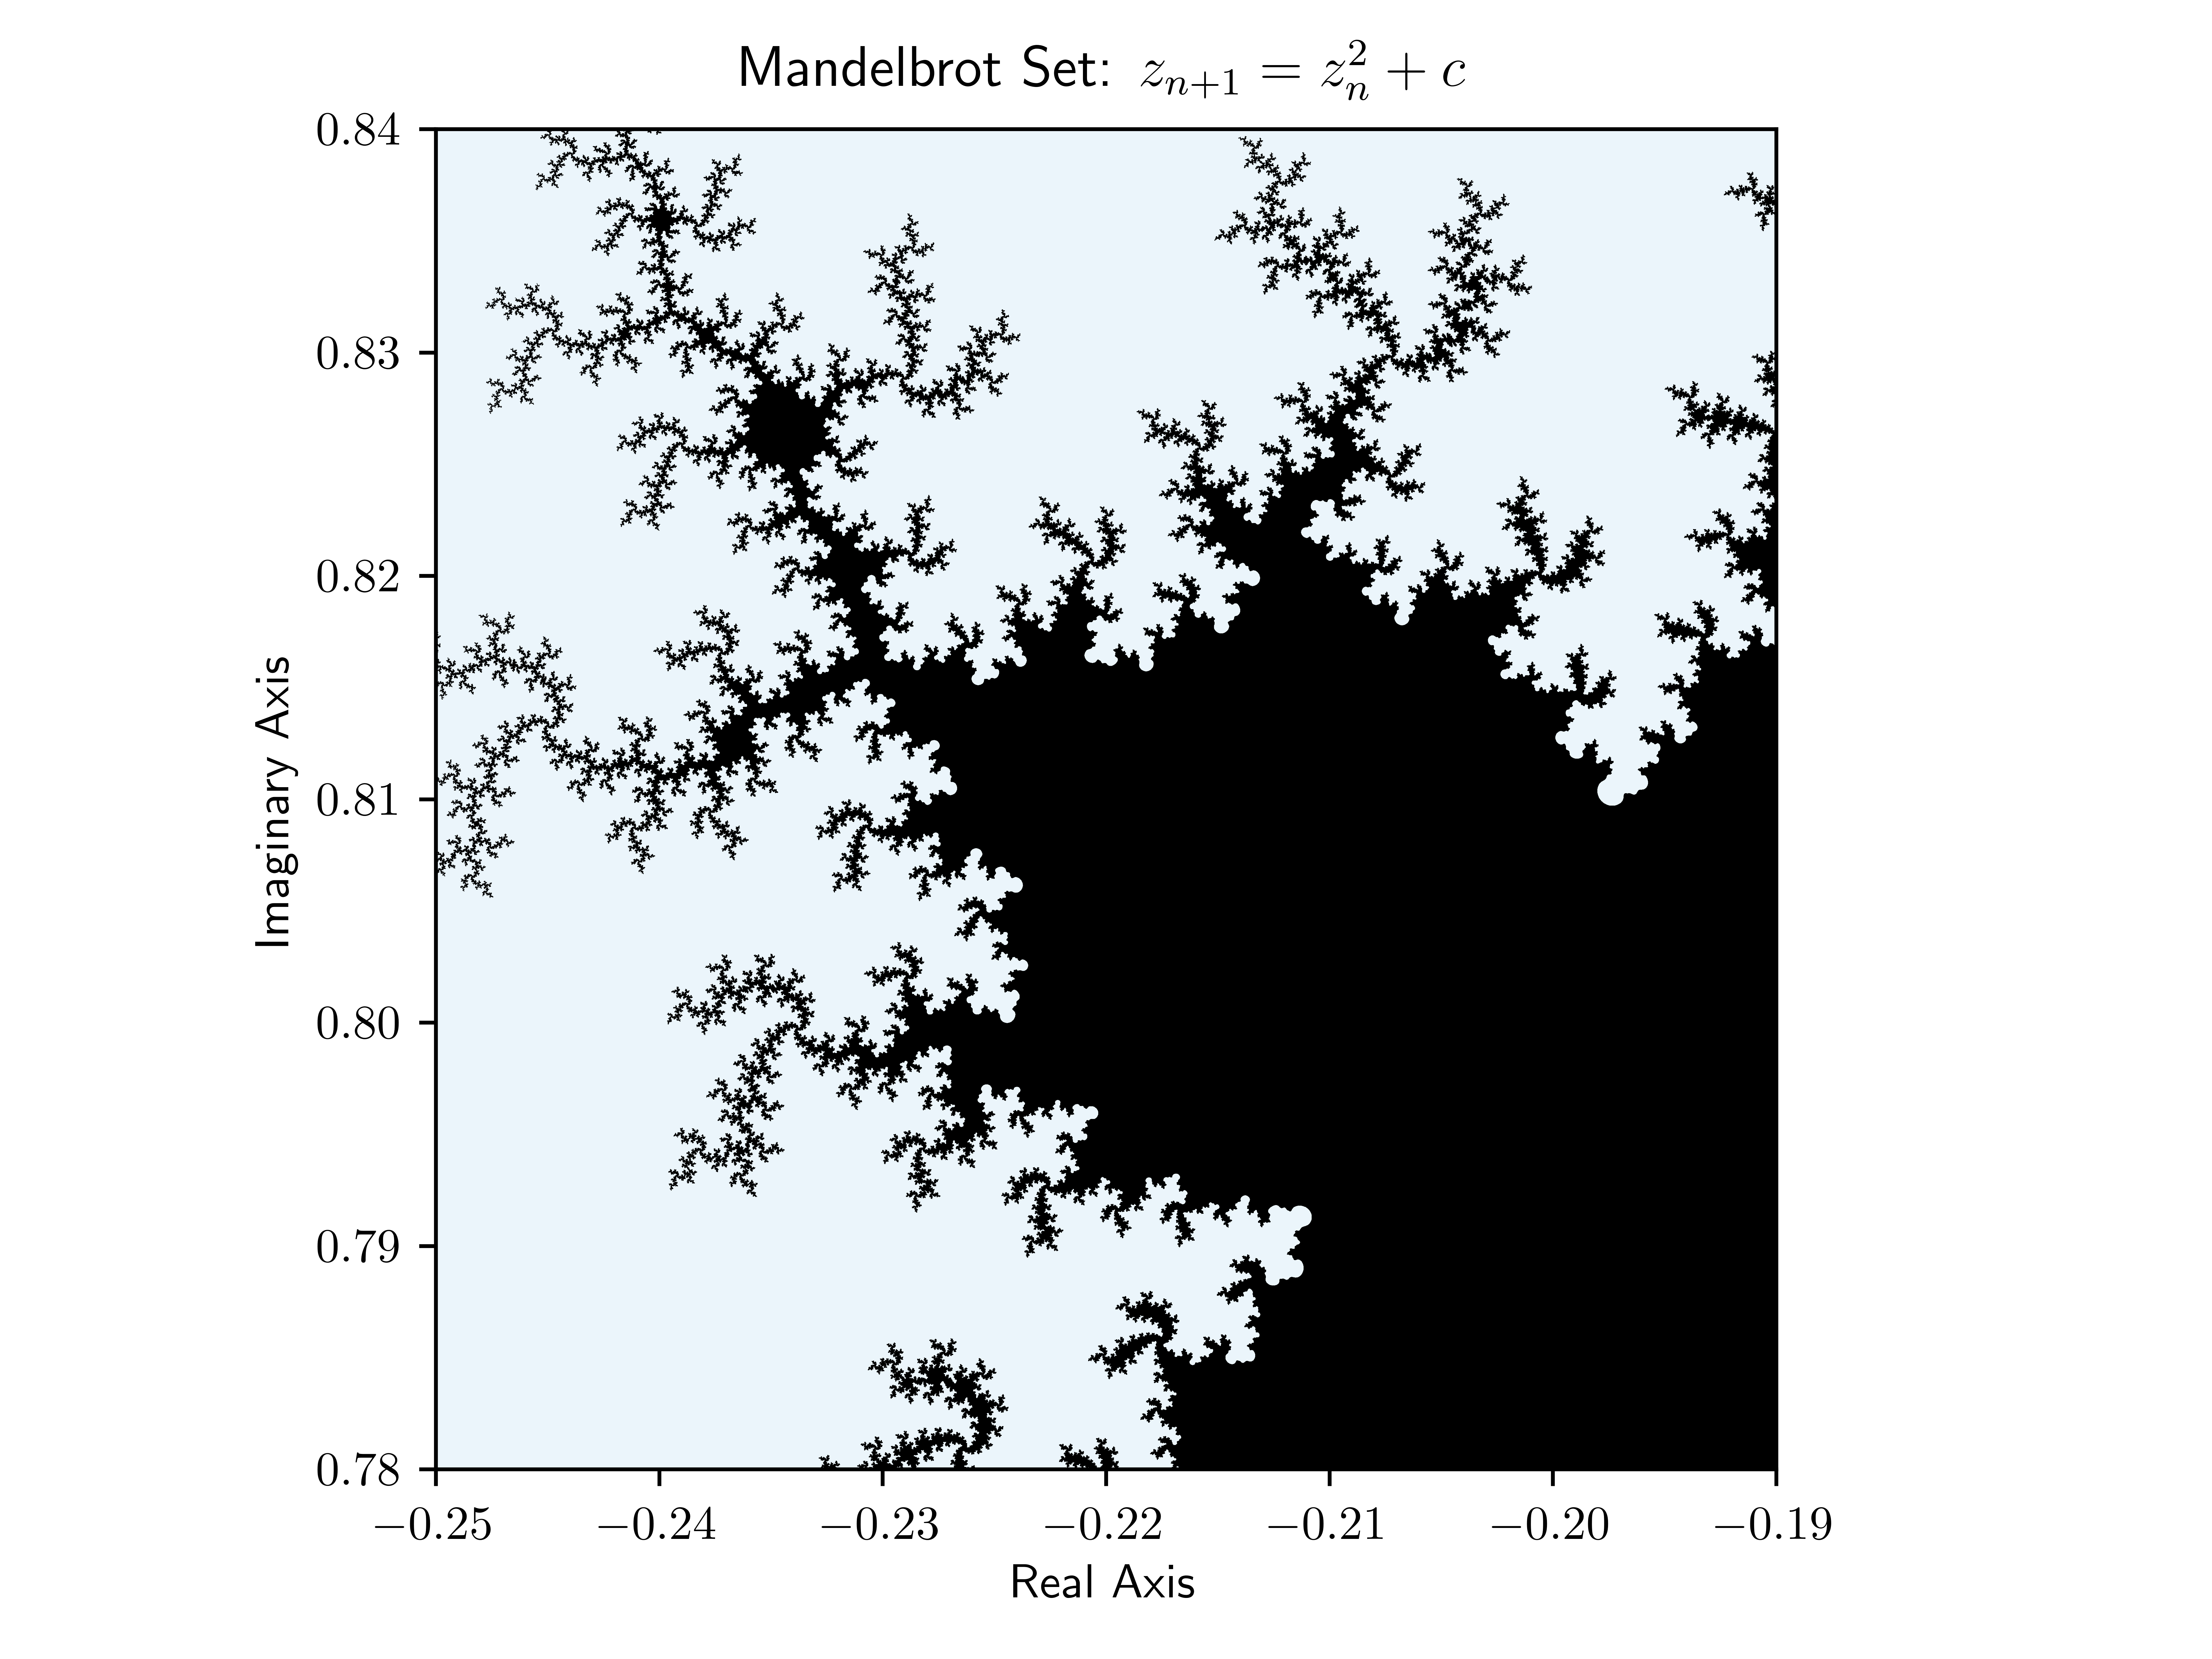
\includegraphics[width = \textwidth]{Images/Mandelbrot_section1.png}
            \caption{Figure 1}
        \end{subfigure}
        \begin{subfigure}{.8\textwidth}
            %\centering
            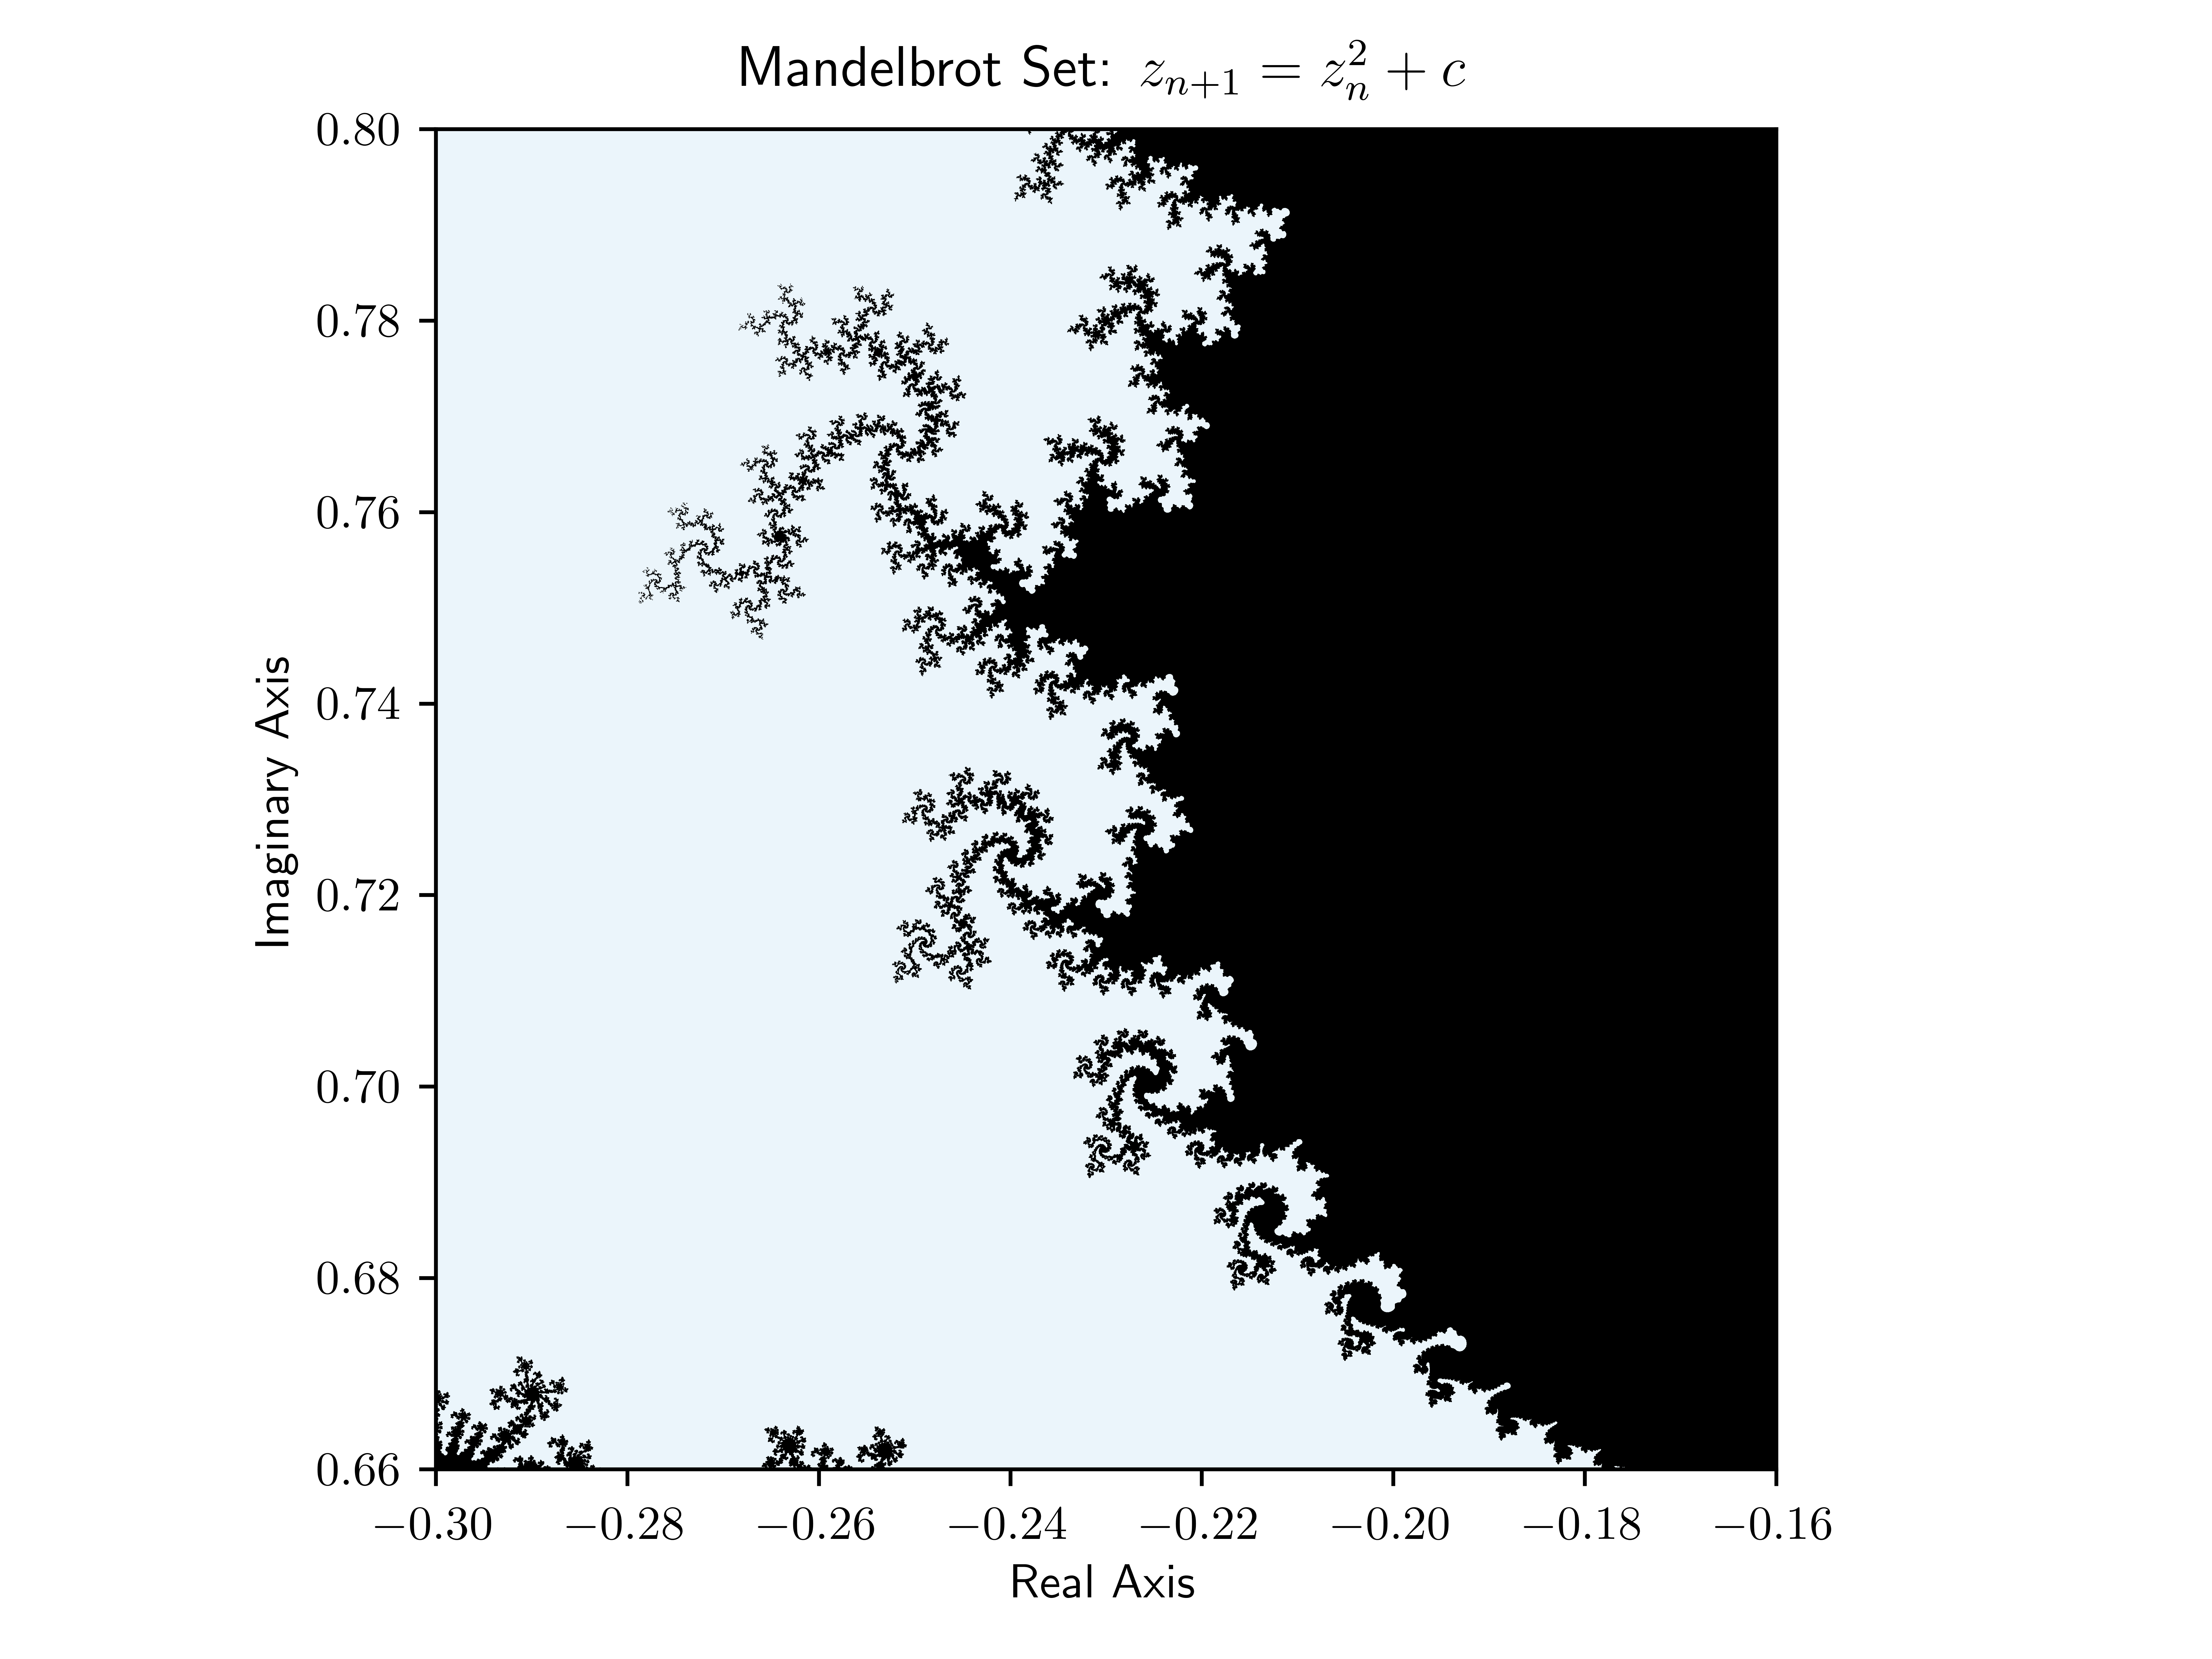
\includegraphics[width = \textwidth]{Images/Mandelbrot_section2.png}
            \caption{Figure 2}
        \end{subfigure}
        % \caption{Zoomed in look at the Mandelbrot Set}
    \end{figure}
    \begin{figure}\ContinuedFloat
        \begin{subfigure}{\textwidth}
            %\centering
            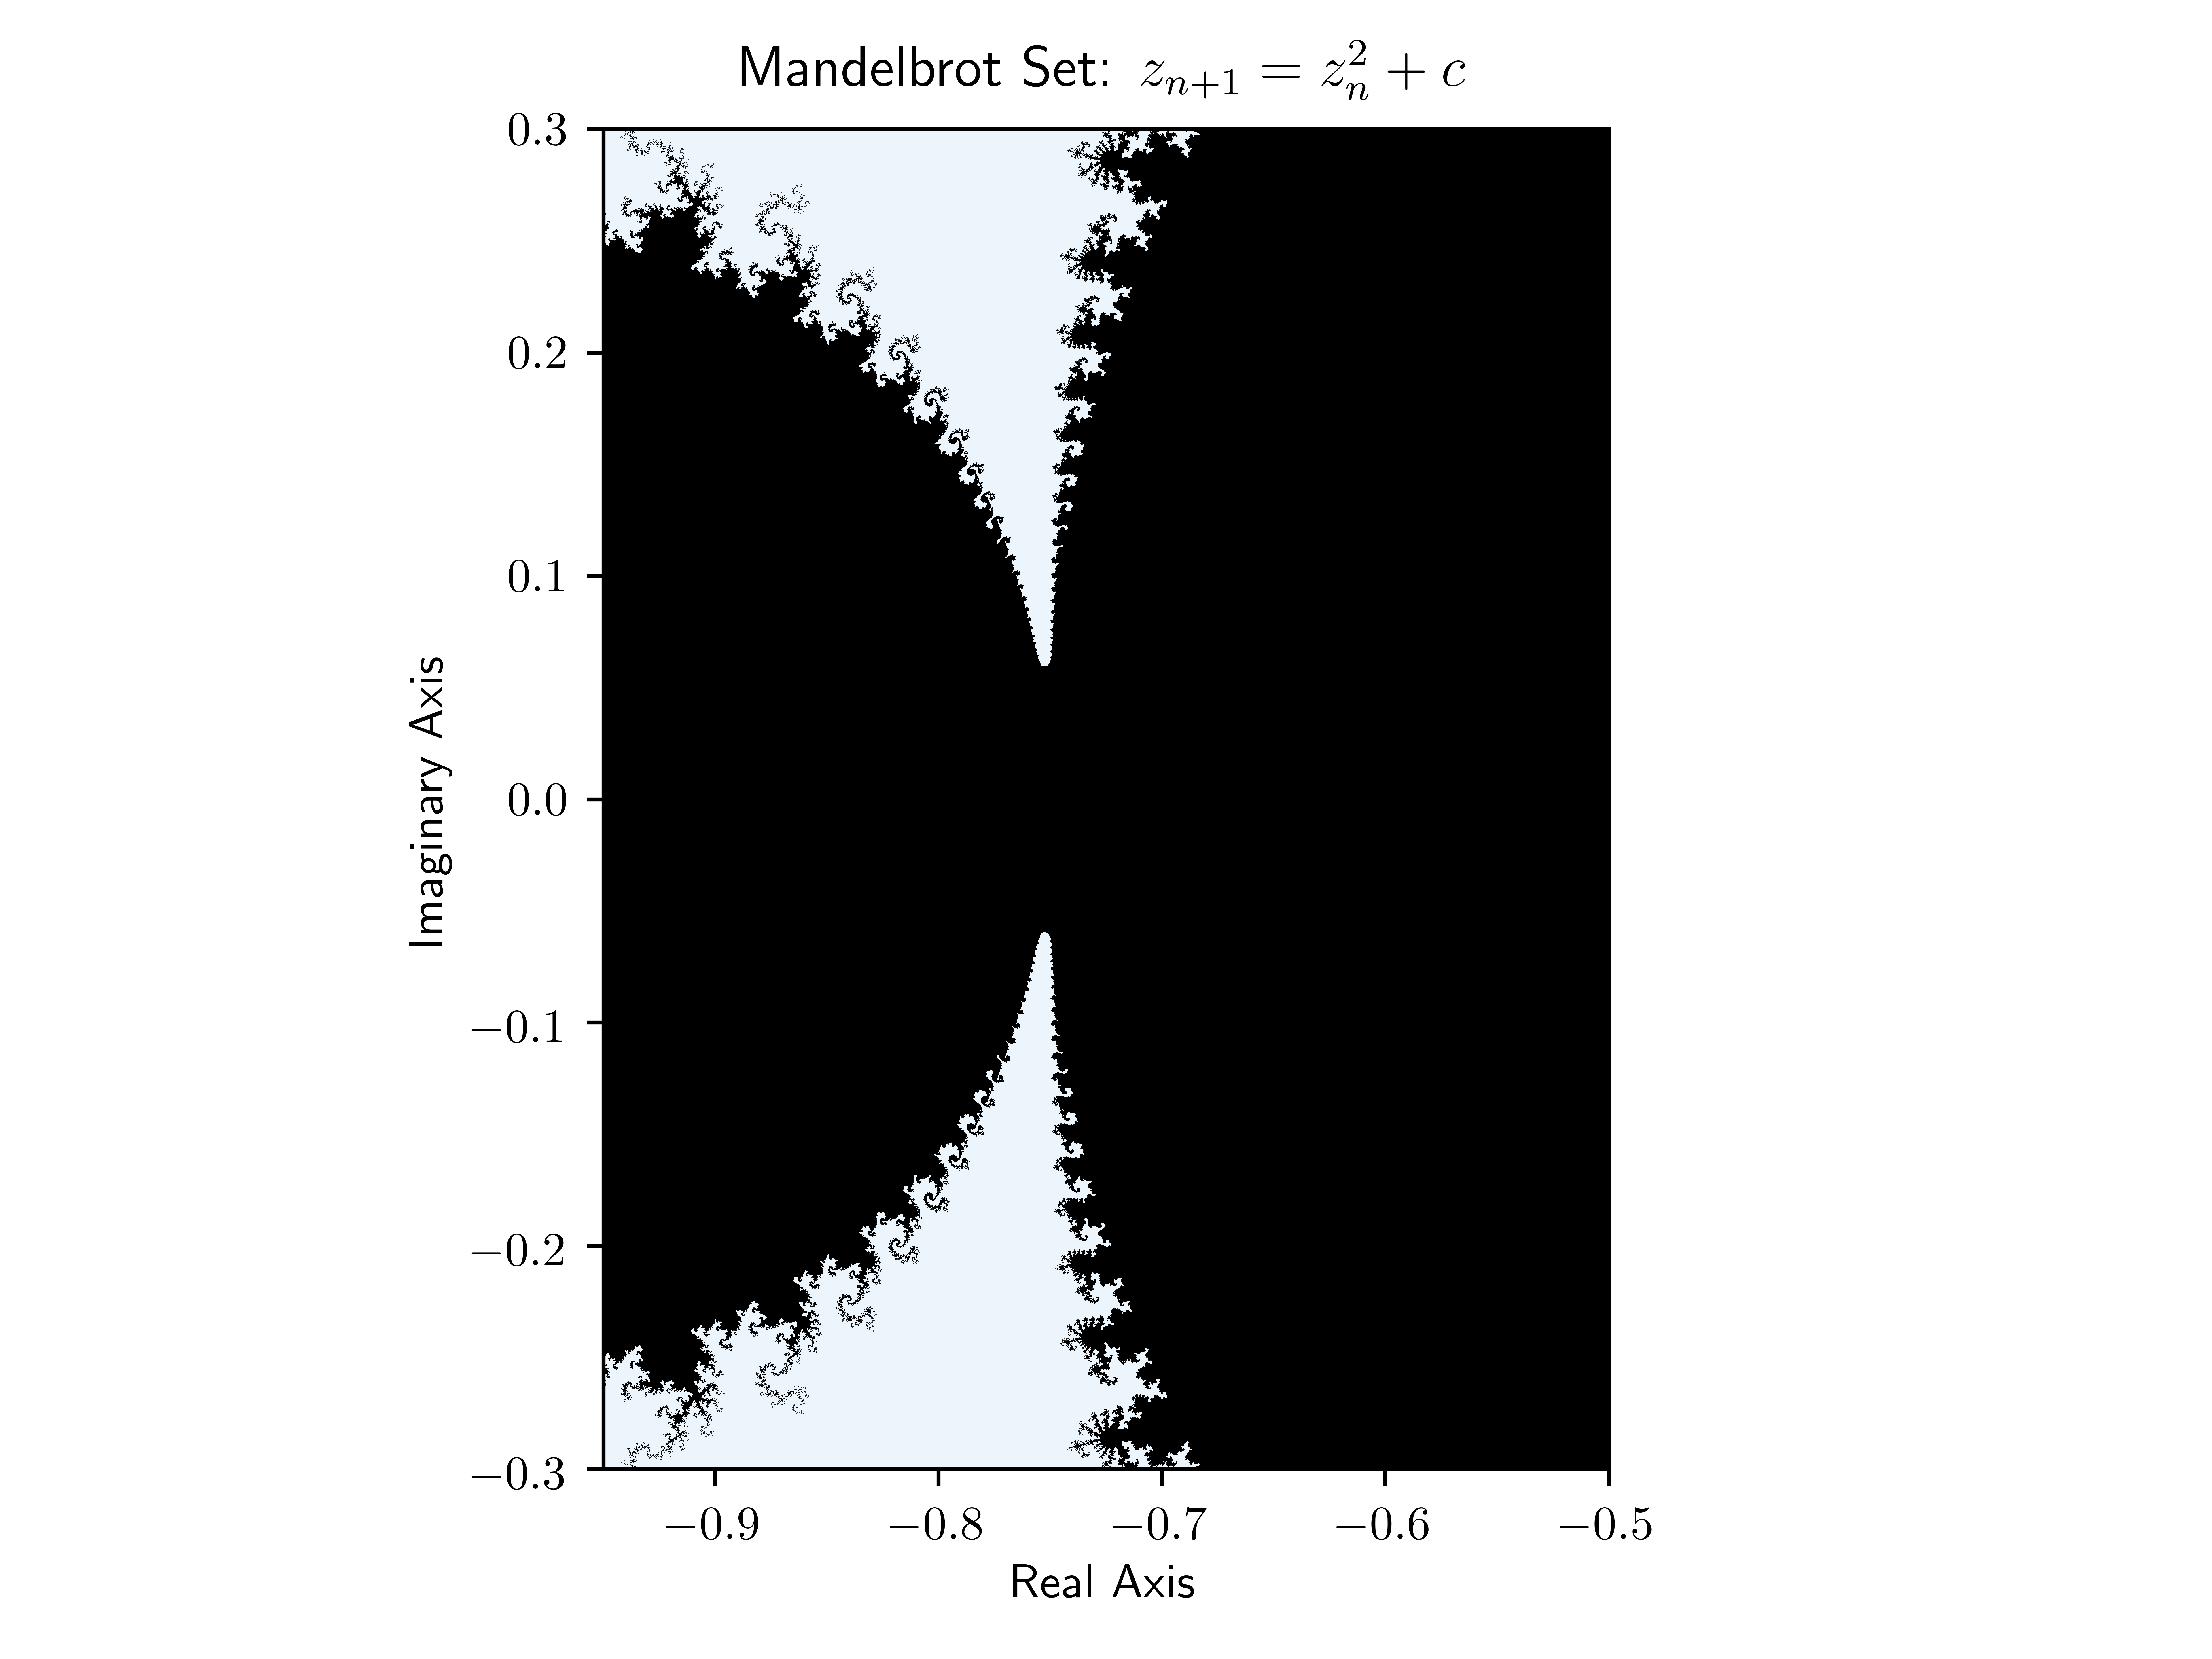
\includegraphics[width = \textwidth]{Images/Mandelbrot_section3.png}
            \caption{Figure 3}
        \end{subfigure}
        \caption{Zoomed in look at the Mandelbrot Set}
    \end{figure}

    \pagebreak


    \section{The Lorenz Attractor}
    Consider the following System of First Order Differential equations.

    \begin{align}
        % \label{eqn:Lorenz_dx}
        \frac{dx}{dt} &= \sigma (y-x) \\
        % \label{eqn:Lorenz_dy}
        \frac{dy}{dt} &= x(\rho-z) - y \\
        % \label{eqn:Lorenz_dz}
        \frac{dz}{dt} &= xy - \beta z
    \end{align}

    % NOTE: for "" use `` "

    This system displays ``sensitive dependence on initial conditions". That is, a seemingly insignificant change in the initial conditions can lead to a dramatically different outcome at a later stage.
    Systems with this property are called \textbf{``Chaotic Systems"}. \footnote[2]{\href{https://www.youtube.com/watch?v=fDek6cYijxI&ab_channel=Veritasium}{Chaos: The Science of the Butterfly Effect - By Veritasium on YouTube}}
    % Chaos: The Science of the Butterfly Effect - Veritasium

    \begin{figure}[h]
        \centering
        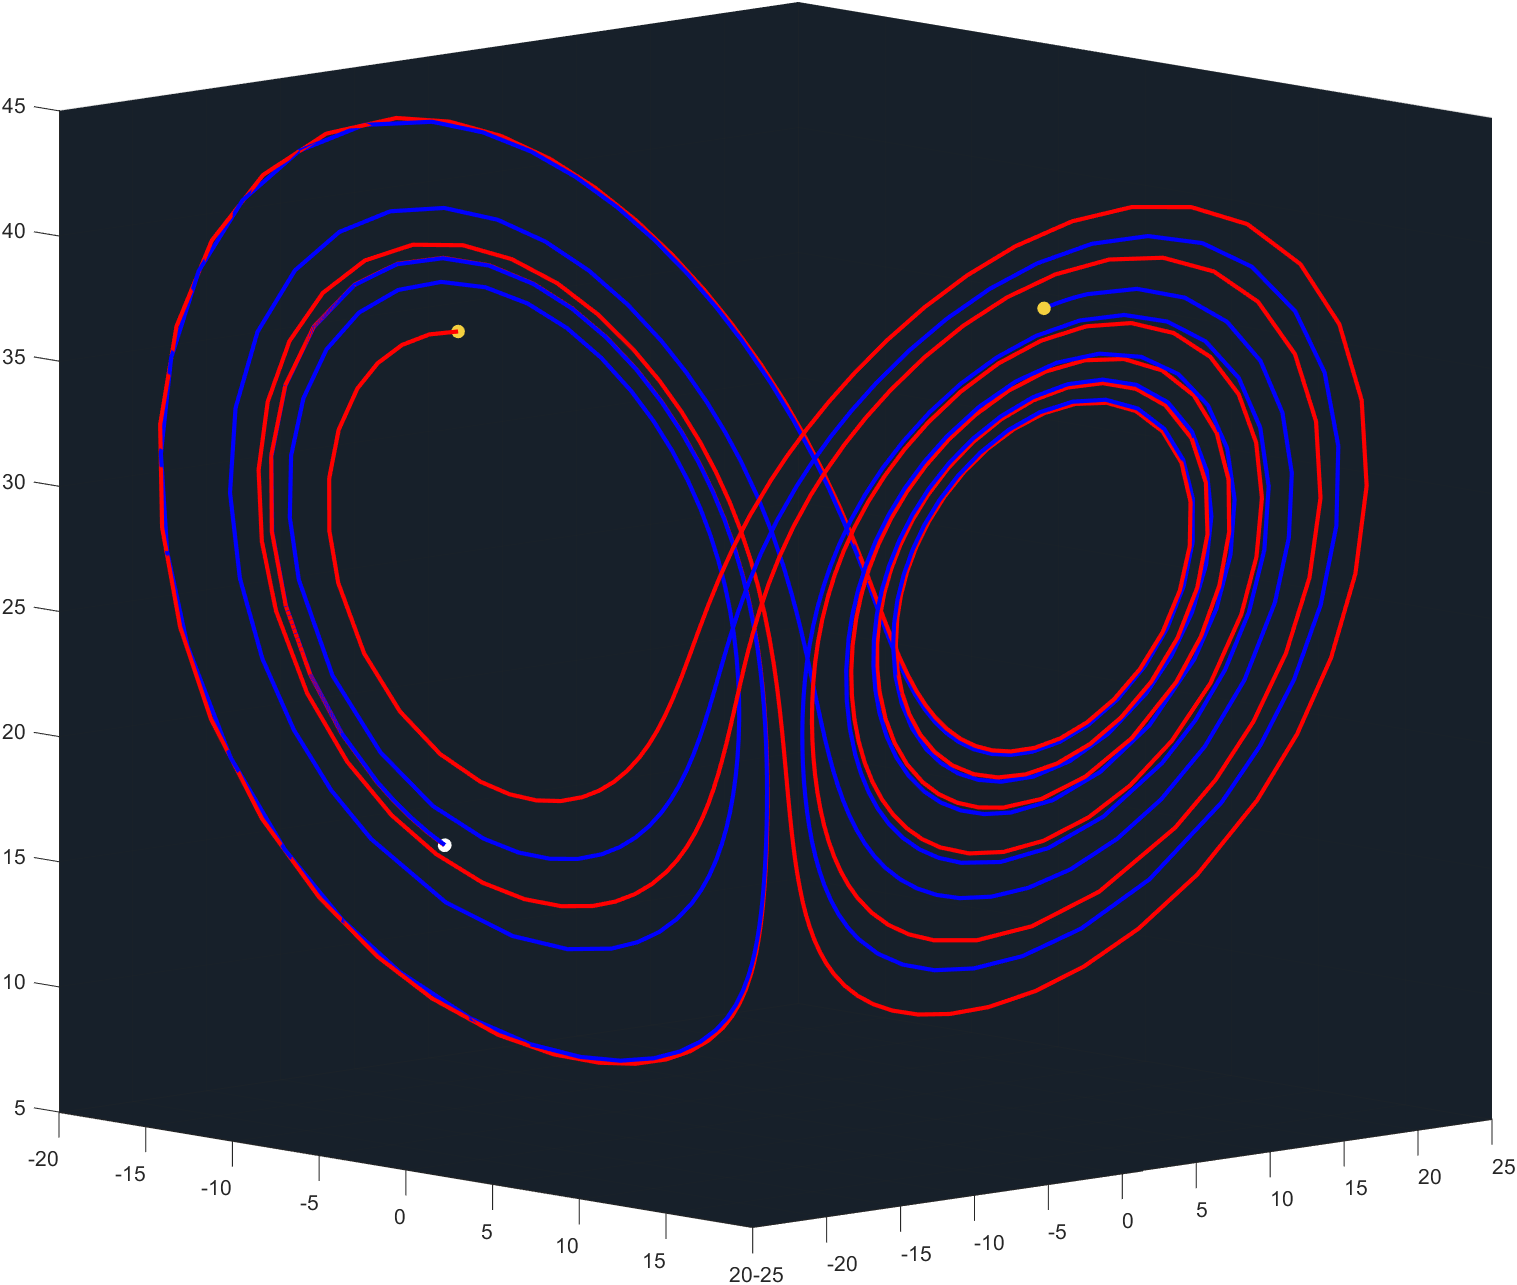
\includegraphics[width = \textwidth]{Images/Lorenz_Divergence.png}
        \caption{Sensitive Dependence on Initial Conditions}
        \label{fig:LorenzDiverge}
    \end{figure}

	As is obvious from Fig.\ref{fig:LorenzDiverge} two initial conditions with a very small deviation from each other(marked in white), evolved into two very different states at a later stage in time(marked in yellow).

    This system also displays another interesting behavior. For a wide variety of initial conditions the system tends to evolve towards a set of states. This set is called an \textbf{``Attractor"}.
    Specifically it settles towards a type of attractor called the \textbf{``Strange Attractor"}.

    Fig.\ref{fig:LorenzAttractor} shows how 2 very close initial states(marked in white) finally settle onto a set, the Strange Attractor(the curve in red and blue).\footnote[2]{For the codes used to generate the plot visit - \url{MYGITHUBPAGE}}

    \begin{figure}[h]
        \centering
        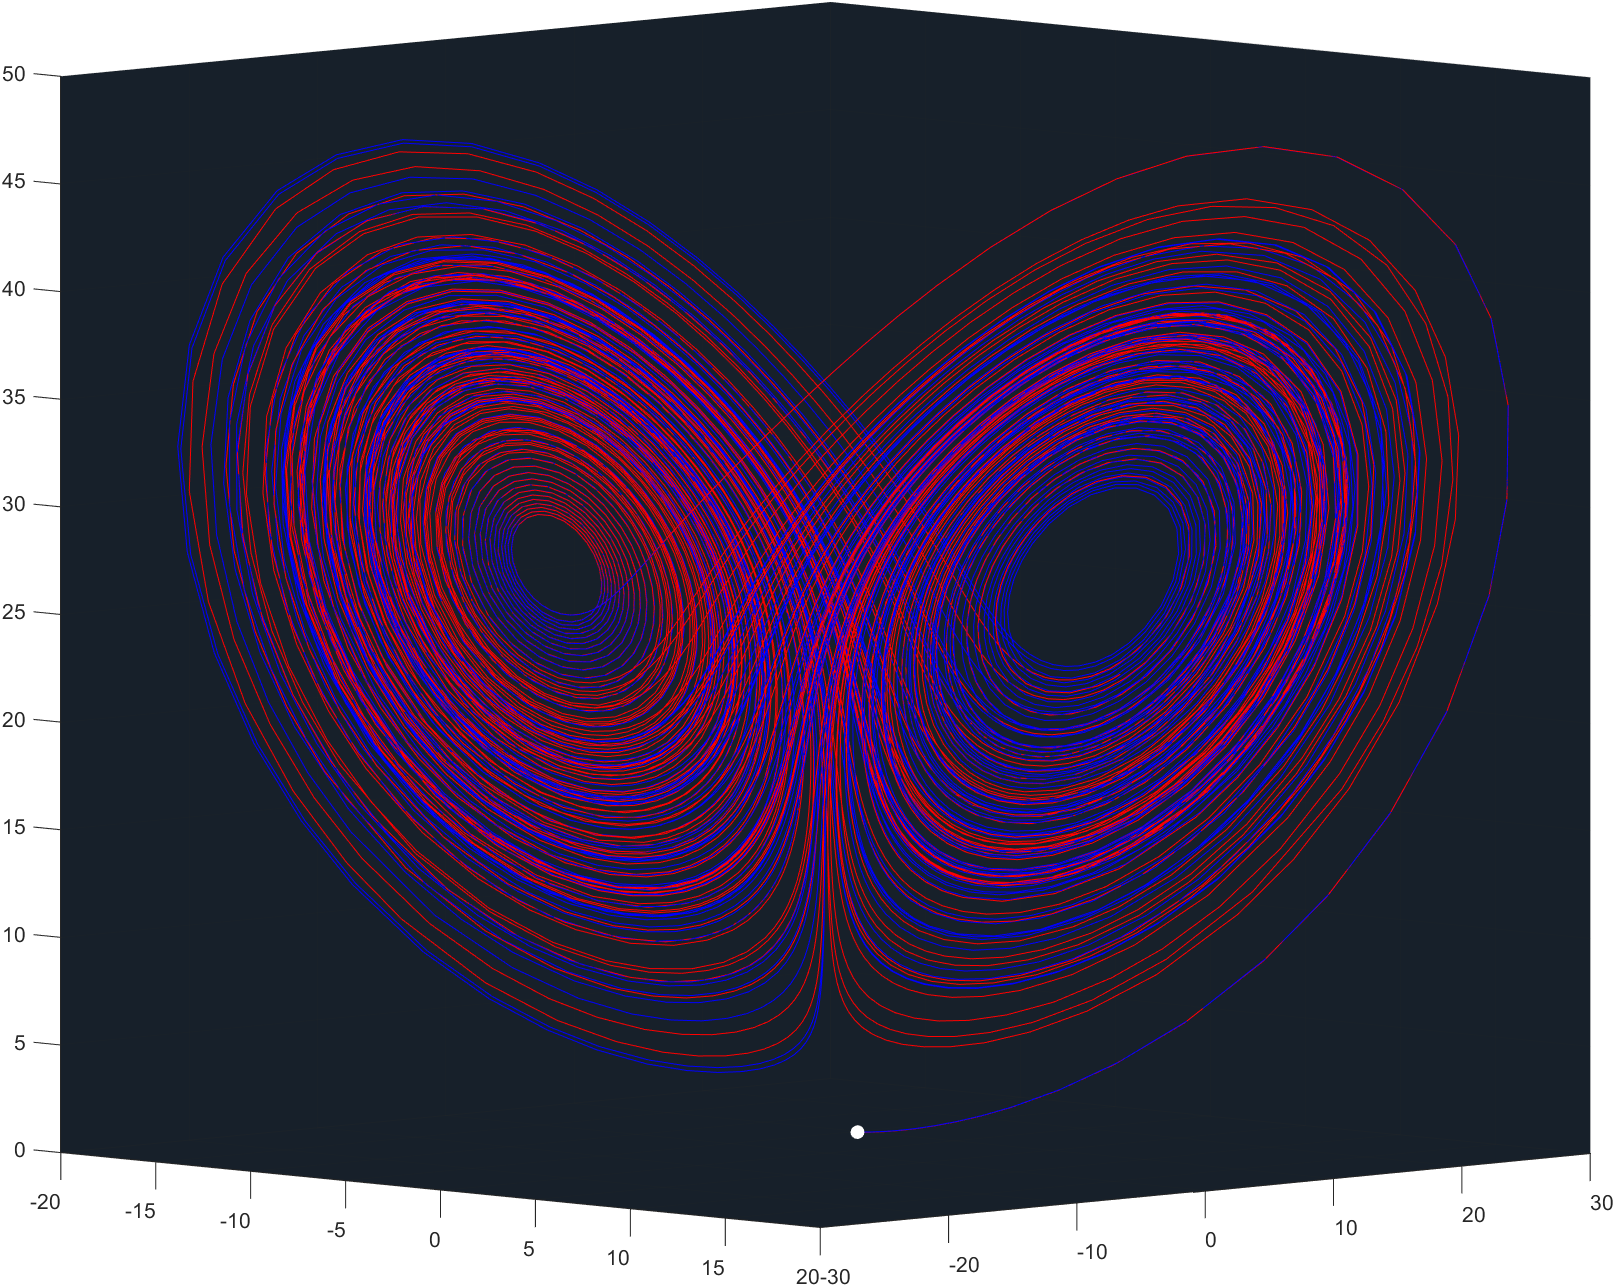
\includegraphics[width = \textwidth]{Images/Lorenz_Attractor.png}
        \caption{The Lorenz Attractor}
        \label{fig:LorenzAttractor}
    \end{figure}

	

\end{document}